\documentclass[a4paper,11pt]{article}
\usepackage{amsmath,amsthm,amsfonts,amssymb,amscd,amstext,vmargin,graphics,graphicx,tabularx,multicol} 
\usepackage[francais]{babel}
\usepackage[utf8]{inputenc}  
\usepackage[T1]{fontenc} 
\usepackage{pstricks-add,tikz,tkz-tab,variations}
\usepackage[autolanguage,np]{numprint} 

\setmarginsrb{1.5cm}{0.5cm}{1cm}{0.5cm}{0cm}{0cm}{0cm}{0cm} %Gauche, haut, droite, haut
\newcounter{numexo}
\newcommand{\exo}[1]{\stepcounter{numexo}\noindent{\bf Exercice~\thenumexo} : \marginpar{\hfill /#1}}
\reversemarginpar


\newcounter{enumtabi}
\newcounter{enumtaba}
\newcommand{\q}{\stepcounter{enumtabi} \theenumtabi.  }
\newcommand{\qa}{\stepcounter{enumtaba} (\alph{enumtaba}) }
\newcommand{\initq}{\setcounter{enumtabi}{0}}
\newcommand{\initqa}{\setcounter{enumtaba}{0}}

\newcommand{\be}{\begin{enumerate}}
\newcommand{\ee}{\end{enumerate}}
\newcommand{\bi}{\begin{itemize}}
\newcommand{\ei}{\end{itemize}}
\newcommand{\bp}{\begin{pspicture*}}
\newcommand{\ep}{\end{pspicture*}}
\newcommand{\bt}{\begin{tabular}}
\newcommand{\et}{\end{tabular}}
\renewcommand{\tabularxcolumn}[1]{>{\centering}m{#1}} %(colonne m{} centrée, au lieu de p par défault) 
\newcommand{\tnl}{\tabularnewline}

\newcommand{\bmul}[1]{\begin{multicols}{#1}}
\newcommand{\emul}{\end{multicols}}

\newcommand{\trait}{\noindent \rule{\linewidth}{0.2mm}}
\newcommand{\hs}[1]{\hspace{#1}}
\newcommand{\vs}[1]{\vspace{#1}}

\newcommand{\N}{\mathbb{N}}
\newcommand{\Z}{\mathbb{Z}}
\newcommand{\R}{\mathbb{R}}
\newcommand{\C}{\mathbb{C}}
\newcommand{\Dcal}{\mathcal{D}}
\newcommand{\Ccal}{\mathcal{C}}
\newcommand{\mc}{\mathcal}

\newcommand{\vect}[1]{\overrightarrow{#1}}
\newcommand{\ds}{\displaystyle}
\newcommand{\eq}{\quad \Leftrightarrow \quad}
\newcommand{\vecti}{\vec{\imath}}
\newcommand{\vectj}{\vec{\jmath}}
\newcommand{\Oij}{(O;\vec{\imath}, \vec{\jmath})}
\newcommand{\OIJ}{(O;I,J)}


\newcommand{\reponse}[1][1]{%
\multido{}{#1}{\makebox[\linewidth]{\rule[0pt]{0pt}{20pt}\dotfill}
}}

\newcommand{\titre}[5] 
% #1: titre #2: haut gauche #3: bas gauche #4: haut droite #5: bas droite
{
\noindent #2 \hfill #4 \\
#3 \hfill #5

\vspace{-1.6cm}

\begin{center}\rule{6cm}{0.5mm}\end{center}
\vspace{0.2cm}
\begin{center}{\large{\textbf{#1}}}\end{center}
\begin{center}\rule{6cm}{0.5mm}\end{center}
}



\begin{document}
\pagestyle{empty}
\titre{Contrôle 1  }{Nom :}{Prénom :}{Classe}{Date}


\vspace*{0.5cm}
\begin{flushleft}
\begin{tabular}{|m{9.5cm}|m{1.25cm}|m{1.25cm}|m{1.25cm}|m{1.25cm}|m{1.25cm}|}
\hline 
\textbf{Compétences} & \begin{center}
\textbf{N.E.}
\end{center} & \begin{center}
\textbf{M.I.}
\end{center} & \begin{center}
\textbf{M.F.}
\end{center}  & \begin{center}
\textbf{M.S.}
\end{center} & \begin{center}
\textbf{T.B.M.}
\end{center} \\ 
\hline 
Je dois savoir produire et utiliser diverses représentations des fractions simples et des nombres décimaux &  &  & & &\\
\hline 
Je dois savoir placer un nombre sur demi-droite graduée &  &  & & &\\
\hline 
Je dois savoir lire l'abscisse d'un point sur une demi-droite graduée &  &  & & &\\
\hline


\end{tabular} 
\end{flushleft}

\textit{N.E = Non évalué ; M.I. = Maîtrise insuffisante ; M.F. = Maîtrise fragile ; M.S. = Maîtrise satisfaisante ; T.B.M. = Très bonne maîtrise}\\




\vspace*{0.35cm}


Les exercices avec le symbole 
\includegraphics[scale=0.4]{trefle.eps} sont à faire directement sur le sujet. Les autres sont à faire sur la copie double.\\


\vspace*{0.35cm}

\exo{1.5} On donne le nombre 982 510. Répondre aux questions suivantes :\\
\initqa \qa Quel est le chiffre des dizaines de milliers ?\\
\qa Quel est le nombre de centaines ?\\


\vspace*{0.35cm}






\exo{4}
\includegraphics[scale=0.4]{trefle.eps} La première ligne de ce tableau est déjà complétée, à vous de finir de compléter le tableau. Chaque ligne correspond à un nombre différent.\\

\renewcommand{\arraystretch}{2.5}

\begin{flushleft}
\begin{tabular}{|p{2cm}|p{5cm}|p{5.5cm}|p{3.5cm}|}
\hline 
\textbf{Écriture décimale} & \textbf{Écriture en toutes lettres} & \textbf{Somme d'un nombre entier et d'une fraction décimale} & \textbf{Une seule fraction décimale} \\ 
\hline 
\begin{center}
 9,103
 \end{center} & Neuf unités et cent trois millièmes & \begin{center}
 $9 + \dfrac{103}{1000}$
 \end{center} &\begin{center}
  $\dfrac{9 103}{1000}$
 \end{center}  \\
 \hline 
\begin{center}
 7,3
 \end{center} & Sept unités et trois dixièmes &  &  \\ 
\hline 
 & Quatre unités et seize centièmes &  &  \\ 
\hline 
 &  &\begin{center}
  $8 + \dfrac{46}{1000}$
 \end{center} &  \\ 
\hline 
\end{tabular} 
\end{flushleft}

\newpage



\exo{4} Dans chacun des cas, écrire sur votre copie le nombre correspondant :\\
\initqa \qa J'ai 54 unités et 7 dixièmes.\\
\qa J'ai 8 dizaines, 34 centièmes et 9 millièmes.\\
\qa J'ai 34 dizaines, 8 dixièmes et 2 millièmes.\\
\qa J'ai 9 643 centièmes.\\



\vspace*{0.1cm}

\exo{1.5} Recopier sur votre copie et compléter avec les symboles $\in$ ou $\notin$ : 

\bmul{2}

\bmul{2}

\initqa \qa E ... [CB)\\

\qa A ... [BF]\\


\qa B ... [CE)

\columnbreak

\qa B ... (AF)\\

\qa A ... [BF)\\

\qa C ... [BE]

\emul

\columnbreak

\includegraphics[scale=0.6]{controle2.eps}


\emul

\exo{3} 
\includegraphics[scale=0.4]{trefle.eps}  Compléter la figure en ajoutant les noms de chacun des six points  nommés dans les indications suivantes : 

\bmul{2}



- $A \in (d_{1})$ et $A \in (d_{2})$ \hspace*{0.5cm} - $B \in (d_{1})$ et $C \in (d_{1})$\\

- $C \in [AB]$ \hspace*{2.5cm}- $F \notin (d_{1})$ et $F \notin (d_{2})$\\

- $D \in (d_{2})$ et $E \in (d_{2})$ \hspace*{0.5cm}- $D \in [AE)$ et $D \notin [AE]$\\



\columnbreak

\begin{flushright}
\includegraphics[scale=0.6]{controle3.eps}

\end{flushright}
\emul


\exo{3} \\

\initq \q Quelles sont les abscisses des points I, G et H ? (Répondre à cette question sur la copie)\\

\includegraphics[scale=1]{abscisses1a.eps} \\

\vspace*{0.25cm}

\q  
\includegraphics[scale=0.4]{trefle.eps} Sur la demi-droite, placer les points : R(4,4) ; P(2,5) et S(7,2).


\includegraphics[scale=0.8]{abscisse2a.eps} \\


\exo{3}  
\includegraphics[scale=0.4]{trefle.eps} On considère les 6 points suivants définis par leur abscisse :

\bmul{2}

\textbf{A}(4,04)\\

\textbf{C}$\left(4 + \dfrac{1}{100} + \dfrac{3}{10}\right)$\\

\textbf{E} a pour partie entière 4 et sa partie décimale vaut 22 centièmes.\\

\columnbreak

\textbf{B}$\left(4+\dfrac{2}{10} + \dfrac{8}{100}\right)$\\

\textbf{D}$\left( 4 + (1 \times 0,1) + (6 \times 0,01) \right)$\\

\textbf{F}(Quatre cent sept centièmes)\\



\emul

$\rightarrow$ \textbf{Placer ces 6 points sur la demi-droite graduée ci-dessous :}

\begin{center}
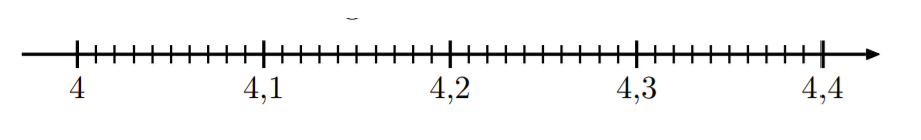
\includegraphics[scale=0.9]{abscisse3.eps} 

\end{center}



\end{document}
